\documentclass{article}

\usepackage[margin=1in]{geometry}
\usepackage[parfill]{parskip}
\usepackage[utf8]{inputenc}
\usepackage{graphicx}

\renewcommand{\familydefault}{\sfdefault}

\begin{document}

\pagenumbering{gobble}
\center

\Huge

Chemistry Instrument Shop

\textbf{
Scientific Glassware Design
}

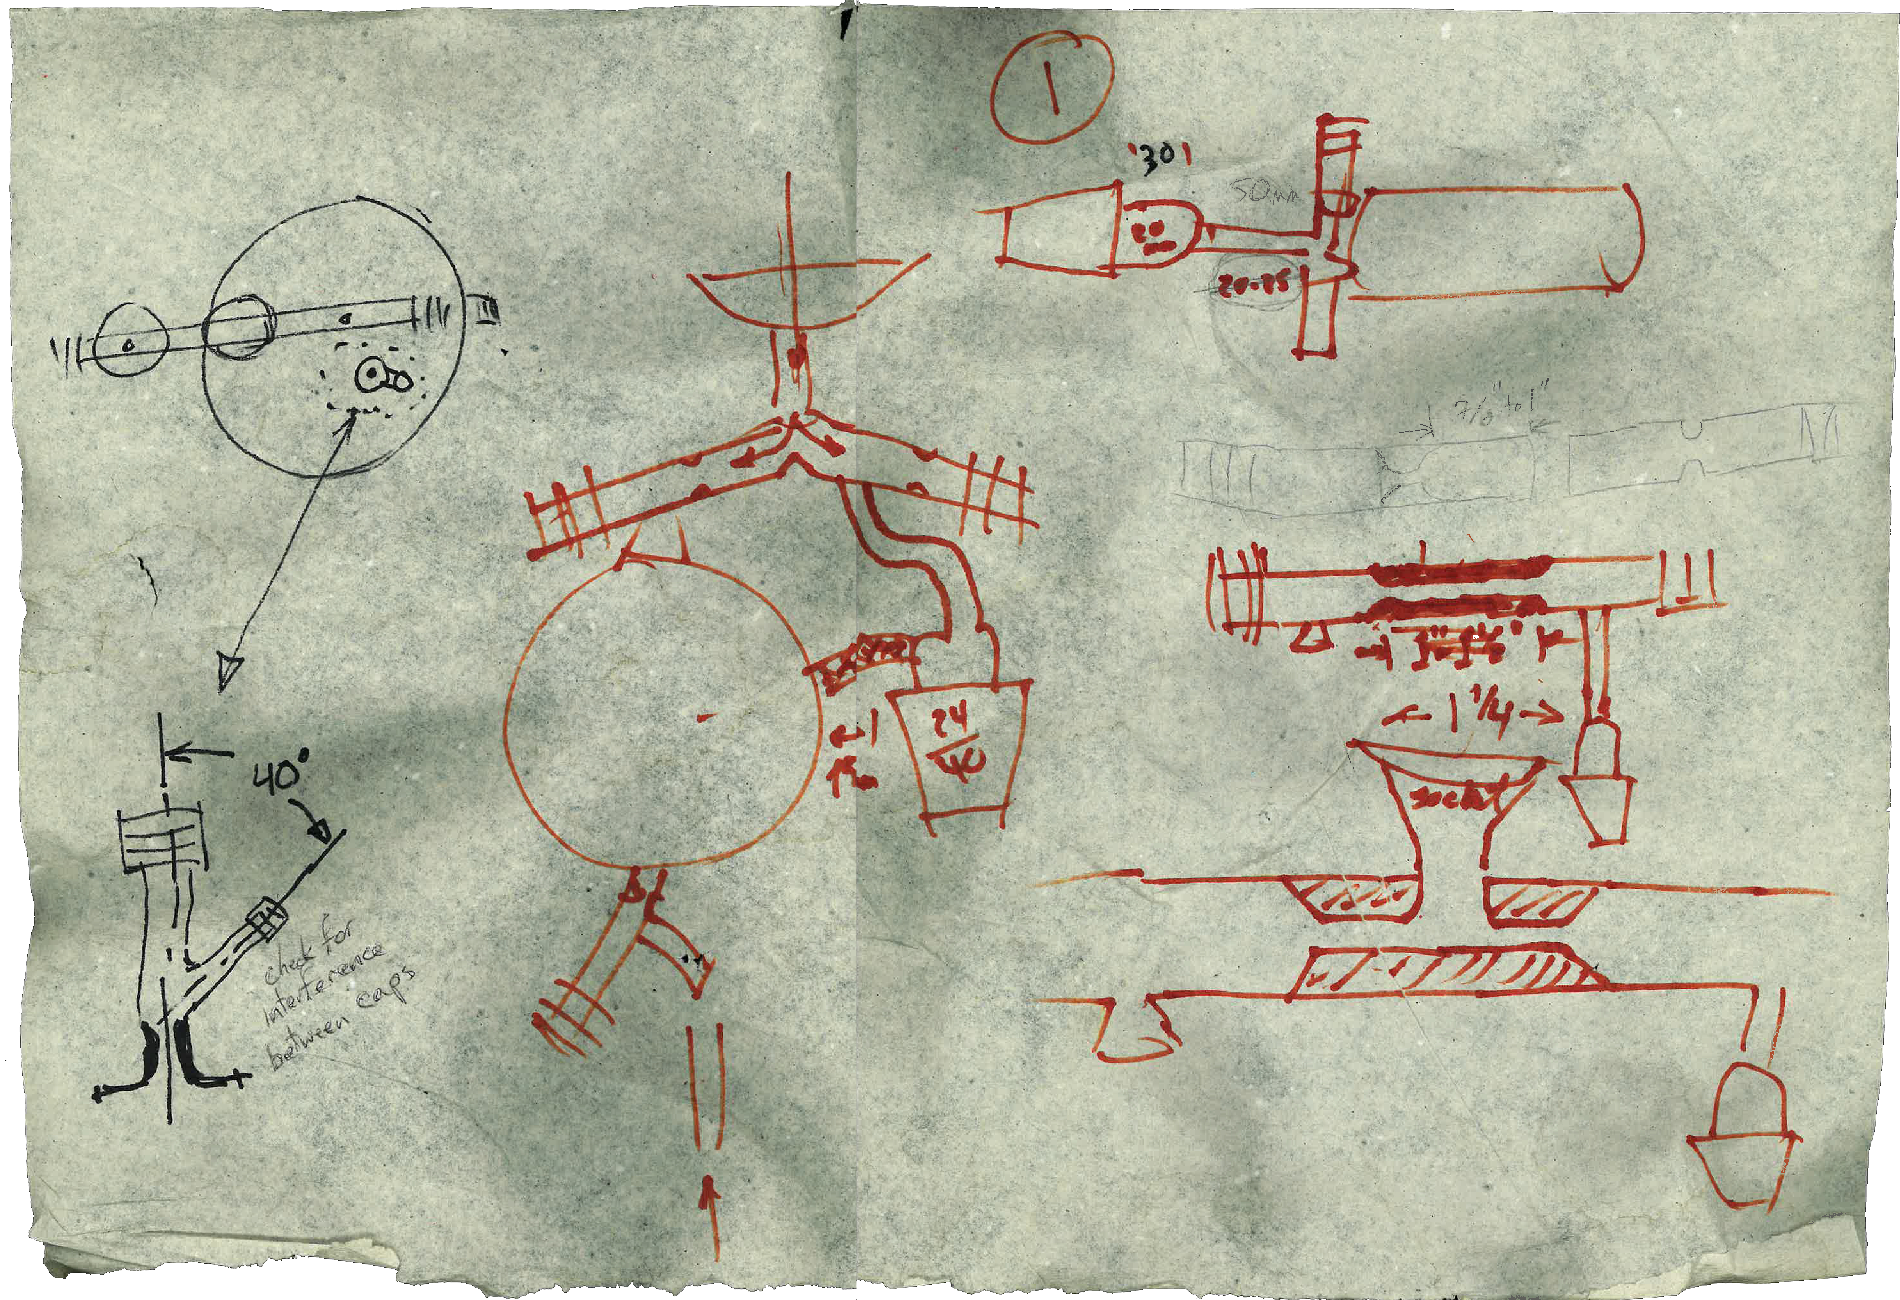
\includegraphics[width=\linewidth]{coverart.png}

{
\LARGE
Learn how to design custom glassware for chemical research. \\
What is possible to build out of glass? \\
What design features make manufacturing difficult? \\
Hear about design and production tricks used in previous projects. \\
Taught by Tracy Drier. \\
}

\vfill

{
\huge
Wednesday June 14, 2 PM \\
Chemistry S307
}

\vfill

{
\huge
Contact blaise.thompson@wisc.edu to participate.
}

\end{document}
